%!TEX root = ../gbctr.tex
%!TEX program = lualatex
\providecommand{\main}{..}
\documentclass[\main/gbctr.tex]{subfiles}
\begin{document}

\chapter{Chip pinouts}

\section{CPU chips}

\begin{figure}[H]
  \centering
  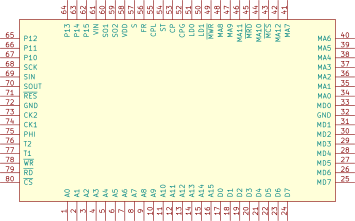
\includegraphics{DMG-CPU-pinout}
  \caption{DMG/SGB CPU (Sharp QFP080-P-1420)}
\end{figure}

\begin{figure}[H]
  \centering
  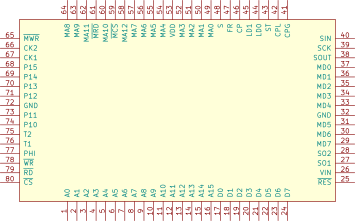
\includegraphics{MGB-CPU-pinout}
  \caption{MGB/SGB2 CPU (Sharp QFP080-P-1420)}
\end{figure}

\section{Cartridge chips}

\begin{figure}[H]
  \centering
  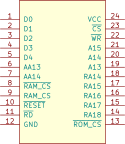
\includegraphics{MBC1-pinout}
  \caption{MBC1 (Sharp SOP24-P-450) \cite{tauwasser_mbc1}}
\end{figure}

\begin{figure}[H]
  \centering
  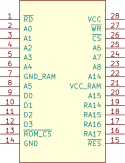
\includegraphics{MBC2-pinout}
  \caption{MBC2 (Sharp SOP28-P-450) \cite{tauwasser_mbc2}}
\end{figure}

\begin{figure}[H]
  \centering
  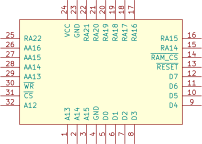
\includegraphics{MBC5-pinout}
  \caption{MBC5 (Sharp QFP32-P-0707)}
\end{figure}

\end{document}
